
Given $AD$ is altitude of the $\triangle ABC$. Therefore

\begin{align}
(\vec{B}-\vec{C})^T(\vec{A}-\vec{D}) = 0
\label{eq:solutions/1/34/eq:a0}
\end{align}


\begin{figure}[!ht] \label{eq:solutions/1/34/fig:triangle_abc}
\centering
\resizebox{\columnwidth}{!}{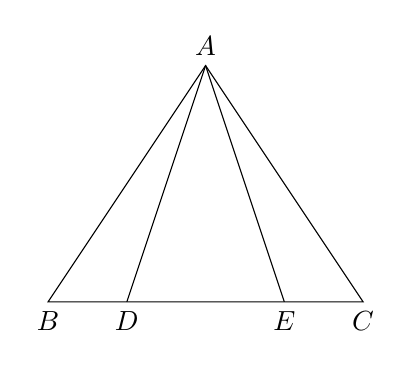
\begin{tikzpicture} 
%	\coordinate (A) at (2, 3) {};
%	\coordinate (B) at (0, 0) {};
%	\coordinate (C) at (4, 0) {};
%	\coordinate (D) at (1, 0) {};
%	\coordinate (E) at (3, 0) {};
%	\draw (A)node[above]{$A$}--(B)node[below]{$B$}--(C)node[below]{$C$}--cycle;
%	\draw (B)node[below]{}--(E)node[below]{$E$};
%	\draw (C)node[below]{}--(D)node[below]{$D$};
	
	
	
	\coordinate (A) at (2,3){};
	\coordinate (B) at (0, 0){};
	\coordinate (C) at (4, 0){};
	\coordinate (D) at (1, 0){};
	\coordinate (E) at (3, 0){};
	
	%Drawing triangle ABC
	\draw (A)node[above]{$A$}--(B)node[below]{$B$}--(C)node[below]{$C$}--cycle;
	\draw (A)node[above]{}--(D)node[below]{$D$};
	\draw (A)node[above]{}--(E)node[below]{$E$};
	
\end{tikzpicture}}
\caption{$\triangle ABC$ with $AD$ as altitude}
\end{figure} 

\begin{multline}
\norm{\vec{A-B}}^2  = (\vec{A}-\vec{B})^T(\vec{A}-\vec{B}) \\
= (\vec{A}-\vec{B})^T((\vec{A}-\vec{D})-(\vec{B}-\vec{D})) \\
= (\vec{A}-\vec{B})^T(\vec{A}-\vec{D})-(\vec{A}-\vec{B})^T(\vec{B}-\vec{D}) \\
= \vec{A}^T(\vec{A}-\vec{D})-\vec{B}^T(\vec{A}-\vec{D})-(\vec{A}-\vec{B})^T(\vec{B}-\vec{D}) 
\label{eq:solutions/1/34/eq:a1}
\end{multline}
Similarly for AC,
\begin{multline}
\norm{\vec{A-C}}^2 = (\vec{A}-\vec{C})^T(\vec{A}-\vec{C}) \\
= (\vec{A}-\vec{C})^T((\vec{A}-\vec{D})-(\vec{C}-\vec{D})) \\
= (\vec{A}-\vec{C})^T(\vec{A}-\vec{D})-(\vec{A}-\vec{C})^T(\vec{C}-\vec{D}) \\
= \vec{A}^T(\vec{A}-\vec{D})-\vec{C}^T(\vec{A}-\vec{D})-(\vec{A}-\vec{C})^T(\vec{C}-\vec{D}) 
\label{eq:solutions/1/34/eq:a2}
\end{multline}
Given AB = AC. Therefore
\begin{align}
\norm{\vec{A-B}} = \norm{\vec{A-C}}
\label{eq:solutions/1/34/eq:a4}
\end{align}
By equating \eqref{eq:solutions/1/34/eq:a1} and \eqref{eq:solutions/1/34/eq:a2}
\begin{multline}
\vec{B}^T(\vec{A}-\vec{D})+(\vec{A}-\vec{B})^T(\vec{B}-\vec{D}) = \\ 
\vec{C}^T(\vec{A}-\vec{D})+(\vec{A}-\vec{C})^T(\vec{C}-\vec{D}) \\
\implies (\vec{B}-\vec{C})^T(\vec{A}-\vec{D})+(\vec{A}-\vec{B})^T(\vec{B}-\vec{D})  \\
= (\vec{A}-\vec{C})^T(\vec{C}-\vec{D}) \quad\text{From \eqref{eq:solutions/1/34/eq:a0}} \\
(\vec{A}-\vec{B})^T(\vec{B}-\vec{D}) = (\vec{A}-\vec{C})^T(\vec{C}-\vec{D})
\label{eq:solutions/1/34/eq:a5}
\end{multline}
Since $\triangle ABC$ is isosceles angle ABD is equal to angle ACD
\begin{align}
\frac{(\vec{A}-\vec{B})^T(\vec{B}-\vec{D})}{\norm{\vec{A}-\vec{B}}\norm{\vec{B}-\vec{D}}} =
\frac{(\vec{A}-\vec{C})^T(\vec{C}-\vec{D})}{\norm{\vec{A}-\vec{C}}\norm{\vec{C}-\vec{D}}} 
\end{align}
By refering the values from \ref{eq:solutions/1/34/eq:a4} and \ref{eq:solutions/1/34/eq:a5}
\begin{align}
\norm{\vec{B}-\vec{D}} = \norm{\vec{C}-\vec{D}}
\label{eq:solutions/1/34/eq:a6}
\end{align}
Therefore BD = DC. In $\triangle ABD$
\begin{align}
\cos{\angle DAB} = \frac{(\vec{D}-\vec{A})^T(\vec{A}-\vec{B})}{\norm{\vec{D}-\vec{A}}\norm{\vec{A}-\vec{B}}} \\ =
\frac{(\vec{D}-\vec{A})^T(\vec{A}-\vec{C}+\vec{C}-\vec{B})}{\norm{\vec{D}-\vec{A}}\norm{\vec{A}-\vec{B}}} \\ =
\frac{(\vec{D}-\vec{A})^T(\vec{A}-\vec{C})+(\vec{D}-\vec{A})^T(\vec{C}-\vec{B})}{\norm{\vec{D}-\vec{A}}\norm{\vec{A}-\vec{B}}}
\end{align}
By refering the values from \eqref{eq:solutions/1/34/eq:a0} \eqref{eq:solutions/1/34/eq:a4}
\begin{align}
\frac{(\vec{D}-\vec{A})^T(\vec{A}-\vec{C})}{\norm{\vec{D}-\vec{A}}\norm{\vec{A}-\vec{C}}} = \cos{\angle DAC}
\end{align}
Therefore angle DAC is equal to angle DAB. Thus AD is the angular bisector of angle A.
